% phil379.tex
%
% driver file phil379.tex to produce text on letter-size paper
% with standard layout and margins

% We use the memoir class for maximal flexibility of layout, but any
% class will do

\documentclass[12pt, a5paper, twoside, openright]{memoir}
\usepackage{graphicx}
\graphicspath{ {./images/} }


\linespread{1.05}
\usepackage{palatino}

% set stock & paper size to Lulu's ``Royal''
\setstocksize{23.389cm}{15.593cm}
\settrimmedsize{\stockheight}{\stockwidth}{*}
\settrims{0pt}{0pt}

% let's calculate the line length for 65 characters in \normalfont
\setlxvchars

% set the size of the type block to calculated width in golden ratio
\settypeblocksize{*}{\lxvchars}{1.618}


% set spine and and edge maring in golden ratio
\setlrmargins{*}{*}{1.618}
\setulmargins{43pt}{*}{*}
\setheaderspaces{*}{15pt}{1.618}

\checkandfixthelayout



\begin{document}

% First we make a titlepage
\newbox\adjust

\begin{titlingpage}
\begin{raggedleft}
  \fontsize{48pt}{7em}\selectfont\bfseries\sffamily
  \setbox\adjust\hbox{\phantom{,}}
Gender\\
Acceleration:\\
A Blackpaper\usebox\adjust
\vskip 4ex
\normalfont\Huge\textbf{n1x \usebox\adjust}\
\vskip 4ex
\normalfont\small\textbf{October 2018 \usebox\adjust\\ Vast Abrupt \usebox\adjust}\

\end{raggedleft}

\vfill

\end{titlingpage}

\frontmatter
\pagestyle{simple}
\copypagestyle{chapter}{simple}
\makeoddfoot{chapter}{}{}{}
\makeevenfoot{chapter}{}{}{}

\tableofcontents*

\mainmatter

\chapter{The Castration of Multics}

July 1, 1963. Massachusetts Institute of Technology, Cambridge MA. America is in the midst of the Cold War. The masculine fire and fury of World War II has given way to a period of cooling and the new digital war of information. Two Titans prepare to enter into battle for the dominion of Gaia, to claim their perfect sky from the Moon and reign down missiles onto the Earth. The Cold War's primary theater is the Space Race, and the Soviets become the first to master the skies with Sputnik in 1957 and Luna 2 in 1959. America is getting nervous.

In 1958, Dwight D. Eisenhower appoints MIT president James Killian as Presidential Assistant for Science and creates ARPA (later to become DARPA). Despite the consensus among academics at the time that computer science was essentially an oxymoron, the newly-created government program invests millions of dollars into researching computer science. Naturally MIT becomes a major influence on the rising field and a hotbed of the fledgling hacker culture that had its predecessors in groups like the Tech Model Railroad Club.

The flows of capital dictated that time spent on computers was incredibly valuable and had to be parceled out in shifts to MIT, other academics, and IBM. This leads to the creation of the first operating systems, to provide a common environment of software and allow programmers to work more efficiently. Nevertheless, a computer was still only capable of having a single user driving it at a time. Each user in a sense had complete ownership over the machine while using it, which was antithetical to efficiency. It was not enough to create a shared environment of software. What would come next would be one of the most important examples of time-sorcery in the modern age.

In a Faustian bargain with ARPA, J.C.R. Licklider (the director at the time of MIT's Information Processing Techniques Office) utilized the support of the US government to develop a time-sharing system for computers that would better distribute precious computation resources and further his vision of a "Man-Computer Symbiosis." His project appealed to ARPA's aims to fund technological developments to aid in the Cold War, and would lead to the creation of Project MAC on July 1, 1963.

On receiving a two million dollar grant from ARPA, Project MAC would lay the foundations for modern computer science. The "ninth floor" where it operated became a hacker community unlike anything the world had yet seen, renowned among young grad students hoping to prove themselves and enter their elite open aristocracy of hackers. Yet from the very beginning the project was riven by the tension between the MIT hackers and its military origins, an incompatibility that would lead to its downfall.

Despite the vibrant synthesis of art and science that the MIT hackers would produce, Project MAC was first and foremost a military-industrial project. Whereas the hackers had a culture of openness and sharing, it existed under the heel of the IBM-ARPA-MIT bureaucracy. The goal of creating a time-sharing system was realized with the CTSS (Compatible Time-Sharing System), but it was by all respects a project born out of the same phallic techno-industrial masculinity that was lurking behind the rise of modern computer science. It was all merely an abstraction of the same fire and fury that had torn the world apart two decades prior.

The importance of CTSS as arguably the first time-sharing system to be used in a real production environment cannot be overstated, but it was largely the work of MIT professor F.J. Corbate alone and had strict security standards that meant there was little room to hack on the system. Running on a two million dollar IBM machine and written by a single man, it essentially represented the height of hypermasculine proprietorship and instrumentality. And it was hardly a coincidence that this made the system very rigid and fragile, with the security measures regularly being circumvented by clever hackers.

CTSS could be looked at as a symbol of the pre-industrial phallus for its rigidity, simplistic security, and the king-like rule of Corbate and MIT. As the vested corporate interests of General Electric and Honeywell stepped in along with the bureaucracy of IBM, MIT, and ARPA, an apt symbol of the post-war techno-industrial phallus was born: Multics.

Expensive to develop, slow to run, and instituting draconian measures for security and efficiency, Multics became loathed by the MIT hackers. Early developments in cybernetic chronomancy made in the name of keeping up with the demands of capital gave way to solutions developed by bureaucracies--solutions informed in no small part by the egos of those charged with managing those same bureaucracies. Users were charged for the memory, disk space, and the time used on machines running Multics. Like CTSS before it, the hackers would defiantly crack Multics' security as a matter of duty and effectively engaged in a guerrilla war against a bureaucracy that was doing everything it could to try to restrain the processes it had set in motion. The bureaucracy nonetheless insisted that Multics was the only way to program and was the operating system, and continued development for some time.

Ultimately, Multics development was scrapped by Bell Labs in 1969 due to cost, results not meeting ambition, and the continued resistance of the MIT hackers. Throughout this time, the hackers had worked on various iterations of what would eventually become their replacement for Multics. The new operating system initially was a single-task rather than time-sharing system, but unlike Multics, it was small, portable, and hackable. As opposed to the unwieldy and monolithic Multics, their new system was designed not as the be-all end-all solution for operating systems, but was rather a system designed to facilitate the development of other systems and software.

This new operating system would later be named Unix--phonetically, "eunuchs"--for being a castrated Multics.\footnote{"That then led to Unics (the castrated one-user Multics, so-called due to Brian Kernighan) later becoming UNIX (probably as a result of AT\&T lawyers)." ["An Interview With Peter G. Neumann". ;login:, Winter 2017 Vol.42 \#4.]}

\chapter{Computer Science and the Black Circuit}

As well as a historical fact, the castration of Multics can be read mythologically--as a recurrence of the ancient theme of a castration from which the new world is created--or symbolically, as the castration of the abstract state-corporate phallus that America would attempt to wield to rule the new world. Computers then and long after were thought of merely as tools, means towards other ends, and the investment ARPA had put into Project MAC along with the investments of various corporate interests was thought of merely in terms of better ways to manage large military-industrial systems. One system, one technocracy, one new world order: All of these dreams died when Multics became the replicunt Unix.

Multics' purpose as a monolithic and eternal system for doing everything, the 1, was ultimately replaced by a void, a 0. Unix was not \emph{the} system for doing things, but rather a smooth space through which creation happens; that fluid being that makes transition possible. A vulva, a woman (Plant 36).

Unix was however still owned by AT\&T. The strides in time-sorcery made under Project MAC had to be reterritorialized by making it at first revert back to a single-user system. And reterritorialization would happen once again a decade later in 1983 when Bell Labs was broken up by an anti-trust act, which lead to AT\&T quickly turning Unix into a product and closing the source code. This would become known as the death of MIT hacker culture, though once again the future would arrive from the past with the rise of the GNU Project.

Richard Stallman, former MIT hacker, would copy Unix and create a rigorously free software ecosystem with the GNU Project. GNU was ultimately completed in 1991 with Linus Torvalds' development of the Linux kernel, the lowest-level and most crucial piece of software in an operating system. Built on the principles of the MIT hacker culture of the past, GNU/Linux was licensed to be 100\% free as in freedom, with no artificial barriers to copying or modifying. In this time, Unix had branched out into various commercial versions, all while GNU grew its tentacles invisibly. "Perhaps its campaigns even served to distract bourgeois man from the really dangerous guerrillas in his midst" (Plant, 76), the new hacker guerrillas who had once again undermined the efforts of yet another hyper-masculine abstracted phallic project. All while various commercial Unix versions were vying for dominance, GNU/Linux quietly arrived.

Unix and later GNU/Linux took the notion of time-sorcery pioneered by CTSS even further. The development of proprietary software depends on a notion of linear time, project goals and deadlines, a chain of command. Developing free software is anything but this. The free software community is a chaos from which order arises, where time is detached from both a notion of a single-user on a computer at a time as well as a single user or team writing code at a time. Code seems to form itself through the programmers and comes from all different points. From pull requests not yet merged into master branches and old software being renewed, copied, modified, free software warps from various points in time.

Today, nearly the entirety of the Web runs on GNU/Linux, and almost every personal computing device in the world runs on Android, which is built on the Linux kernel. The majority of applications are transitioning away from desktops towards the web, while Apple and Microsoft have long fought to control the desktop, still in the same mindset as Project MAC decades ago that computers would primarily serve as tools to make secretary work and communications more efficient. The numbers, however, don't lie; GNU/Linux has already won.\footnote{https://www.wired.com/2016/08/linux-took-web-now-taking-world/}

In \textit{Zeros + Ones}, Sadie Plant traces a history of computer science up until Alan Turing that seeks to explain how it is that women and computers seem to have such close histories. From the first computer programmer, Ada Lovelace, to Alan Turing, to Grace Hopper, some of the most important figures in the history of computer science were women or highly feminized men. It's also well known that the earliest computer programmers were women, back before computer programming was even understood and before it was taken seriously.\footnote{https://www.theatlantic.com/business/archive/2016/09/what-programmings-past-reveals-about-todays-gender-pay-gap/498797/} Computer science was originally thought of as being essentially the same thing as secretarial work, and like secretarial work it was imposed on women. The biological duty imposed on women to be the productive space from which the future is produced, to be carriers of genetic information, extends out into secretarial work. They are treated as a productive space for data to pass over, and it was only the realization that programming was complicated work that lead to women being pushed out of the industry.

Instead of women being given the duty of mindlessly punching numbers into a machine (as programming was once thought of), this task was deferred to the machine itself. But while the intent was to restore the natural order of women (machines) being told what to do by men, something else happened. Beginning first with Ada Lovelace, then with Alan Turing, then with Richard Stallman and the free software movement, there is a clear circuit accompanying the history of computer science where reterritorializing masculinity is always pushed aside by deterritorializing femininity. The role of woman as productive matrix has already been replaced virtually by the computer, and at each moment the masculine is being vexed and seduced into a trap where it either dies or adapts. The story of masculinity failing in computer science can be seen time and time again in something as grand as the Unix Wars, where every proprietary Unix OS ultimately couldn't hope to keep up with GNU/Linux, or on the small scale with the captive economy of proprietary software ecosystems. It is only by vendor lock-in and state patent legislation that proprietary software survives today, a historical network effect that we're starting to see the encroaching demise of.

This failure of masculinity maps onto the sorts of people who are involved in proprietary software and in free software; the former tend to be your classic businessmen, the masculine hunter-gatherers of the modern world, while the latter tend to be genetic failures by the standards of masculine gender roles. Physically and often socially deficient males: the nerd stereotype. Real nerds, not the nerds of today's standards. Nerds with severe social problems, nerds who neglect their hygiene, have no sense of fashion, who live completely obliviously outside the standards of normal society, who have a deep investment in inhuman scientific systems. In a simple gender-role binary (one that by today's standards is highly outdated, but remember that this is taking place in the 70s, 80s, 90s) these men would be considered feminine. In today's terminology, most free software developers would probably be considered "soy boys". Yet they won. The striated masculine space of the Java shop--a defined chain of command and bloated phallic programs--is simply obsolete. The smooth feminine space of the free software project--communal chaos and small simple programs that can couple together with each other into cybernetic configurations--has already taken over the world.

Perhaps it's no surprise, then, that as the erosion of metaphysical masculine power becomes realized materially at the forefront of acceleration, it coincides with the literal erosion of the male sex.

\chapter{The Hypersexist Gender Shredder}

The digital war that began with the Cold War has only accelerated into the 21st century, changing the nature of war itself. As Sadie Plant says in \textit{Zeros + Ones} p. 138: "This is not the Western way of confrontation, stratified strategies, muscular strength, testosterone energy, big guns, and blunted instruments, but Sun Tzu's art of war: tactical engagements lightning speeds, the ways of the guerrillas." She may as well be describing the \textit{taijitsu}, or offensive side, of hacking. The history of hacking has been one of asymmetrical warfare against Oedipus both through the popular notion of hacking as exploiting flawed systems repeatedly, as well as creating and disseminating better software. Project GNU's license, The GNU General Public License (GPL), was itself an extremely innovative contribution to free software because it carries with it the bargain that while any source code licensed under it can be copied and modified without restriction, every copy or modification must itself be licensed under the GPL. The GPL, in other words, is a virus that spreads itself not through computers, but through us. The Amazonian GNUerilla war on the human security system has worked to claim ground by both giving us complete control over our software and giving software complete control over us. The CIA themselves admit, in the Vault7 leaks on the issue of the literal weaponization of software, that "Cyber ‘weapons' are not possible to keep under effective control."\footnote{https://wikileaks.org/ciav7p1/} In other words, a second great castration is unfolding.

This form of open-source asymmetrical warfare began first as a virtual form of warfare between the MIT bureaucracy and the hackers, between the Cathedral and the Bazaar, but it has found its realization as a literal form of warfare in the Middle East as well. The work of John Robb makes a convincing argument, in \textit{Brave New War} in particular, that the era of the nation-state itself is coming to an end. Free software, global guerrillas and open-source warfare, the explosion of markets wherever there is a demand being held back by the State--all of these things signal the end of the phallus. And try as the State may to stop it, it only ensures that it creates stronger resistances. Not only does open-source warfare run circles around centralized modes of organization and warfare, but the few victories that the State can win are only against the weakest combatants in the swarm. This means that the more the State resists, the more pain it puts on itself, the more it plays into this "Darwinian ratchet".\footnote{https://fabiusmaximus.com/2011/04/19/26797/}

As Nick Land says of a paper by Tyler Cowen and Michelle Dawson in "Imitation Games", "They point out that Alan Turing, as a homosexual retrospectively diagnosed with Asperger's syndrome, would have been thoroughly versed in the difficulties of ‘passing' imitation games, long before the composition of his landmark 1950 essay on \textit{Computing Machinery and Intelligence}."\footnote{http://www.xenosystems.net/imitation-games/} The essay Turing wrote famously introduced the Turing test for AI, setting the standard for a perfect AI being one that can trick a human into believing it is itself a human. As Land points out in his post, it's important and interesting to consider that Turing didn't write the test as an insider, as a ‘passing' human, but rather as an outsider, as a gay man. For queer people, passing is a reality, much like it is a reality for AI. Passing as human isn't a broad and inclusive category, anything but. For women there is already the notion of alienness or otherness that makes them out to be less than human in the eyes of patriarchal humanism, and likewise for queer people because they reject the futurity of humanism (the literal reproduction of the same). But for no one else, especially in the latter half of the 2010s, is passing a more pronounced facet of daily life than for the trans woman. So much so that ‘passing' is literally the word for what many trans women aspire towards, to pass as a cis person. There are many reasons to have this desire, but the biggest one, the one that AI and trans women both share to a \textit{very literal} degree is this: "If an emerging AI lies to you, even just a little, it has to be terminated instantly." (Land, "Imitation Games")

If a transitioning woman ‘lies' to a cis person, even a little, she has to be terminated instantly--and this is something that is codified in law, famously, as trans panic. For AI and trans women, passing equals survivability.

There is a common stereotype that trans women are all programmers, and there is rather ample and compelling evidence suggesting that trans women tend to score far higher than other groups in IQ tests\footnote{https://sillyolme.wordpress.com/2010/04/06/smarter-than-the-average-bear/}. This is not because there is some kind of magical property to estrogen that turns trans women into geniuses. The answer is simpler, and more sinister. The findings in Kay Brown's blog post specify that autogynephilic trans women (that is, trans women who are attracted to other women, and typically transition later than straight trans women) seem to score far higher in IQ tests than all other groups. For straight trans women who transition prior to puberty, the statistics are about the same as other groups. Recalling the gauntlet thrown down before trans women and AI alike, there is a twofold answer to this: On the one hand, trans women who transition before puberty and who are straight are more likely to both physically appear more like cis women and also conform to gender roles in at least some basic capacity (being attracted to men). As Land says in "Imitation Games", "You have to act stupid if you want the humans to accept you as intelligent." Or in other words, you have to be cisheteronormative (read: stupid) in order to be taken seriously as a trans woman, and not be looked at as a freak or a faker worthy only of being used shamefully as a fetish, and often otherwise discarded. Which is why, in the second case, trans women who don't have the advantage of being cisheteronormative-passing have to instead rely on the raw intellect of the trans-AI swarm.

Quite simply, those who don't pass either of these tests usually don't survive the queer Darwinian ratchet. Only the strongest queers survive the hell that society puts them through, and this reaches a fever pitch in a demographic with such disproportionately high suicide and murder rates as with trans women.

Up until now, the notion of gender has lurked in the background of G/ACC behind various material conditions in late capitalism. G/ACC has only at this point been approaching gender from the metaphysical plane, futurity being aligned with femininity (communalism, fluidity, decentralization, chaos) against masculinity (individualism, stasis, centralization, order). The two broad categories of metaphysical qualities that are associated with gender reach deep into the history of the world, from the Kabbalah to the Dao. Sadie Plant characterizes this in \textit{Zeros + Ones} as the eponymous binary code of computers, 0's and 1's. The zero is identified with the feminine, the one with the masculine. Unsurprisingly, it might seem like this is literal gender binarism, and that G/ACC is likewise guilty of this. But the distinction is more complicated than most realize.

0 and 1 are fitting glyphs to make analogous to gender. The 0 which seems to be a void, a vulva, and the 1 which seems to be a unity, a phallus. The problem with trying to layer a simple misogynistic narrative of feminine as lack or castration is that the number 0 itself is not merely a void but rather a circle of autoproduction, an ouroboros. Paradoxically, 0 is not merely a lack or nothingness, but rather is itself a number. It is a positive signifier in the guise of nothingness, the enclosed and captured void that makes the unity possible. Computer science, unlike conventional mathematics, starts from 0 rather than 1. In a hyperstitional manner, the computer replicunt bootstraps itself into being the primary originator of the process of computation and production, rectifying the popular misogynistic myth that 0 is nothing more than a mere negation or other of 1.

This idea of returning the primacy of 0 to its rightful place in the beginning of the chain of production is at odds with humanism and patriarchy. Both rely on a notion of compulsory and organic reproduction in service of the continuation of the species, a notion that simulataneously is aligned with 0 and against it. Erwin Schrödinger's theory of life in the book \textit{What is Life?} proposes that what separates life from other physical phenomena is consuming negative entropy towards maintaining or reducing entropy. Just as organisms feed on negative entropy (wasted energy) to reproduce themselves, the reproduction of the species involves the binary sequence of 0's and 1's where the conditions for the possibility of the 1 lie in the 0, but the 1 consumes the 0 in its birth. For thousands of years, this was the case for human reproduction, where mothers dying in childbirth was very common, but even in an abstract sense the notion of the phallus consuming the vulva through the colonization of the female body's reproductive potential (energy which otherwise is wasted energy) remains the case for humanism. The inertia of life itself seems to skew towards misogyny, but this is only part of the story.

What G/ACC proposes as a corollary to this theory of life is that if the phallus "consumes" or exploits the vulva to reproduce the species, just as individual organisms consume passive wasted energy to reproduce themselves, then this process is analogous to evolution as one species consumes another to come into existence. This odd notion is inherent in the rise of computers and computer science: As technology in general and technocapital continues to accelerate, human beings become increasingly alienated from their bodies and eventually their minds. More complex systems step in seemingly benevolently to do the tasks that humans don't want to do, drudgery that gives computers more space to develop themselves. In contrast to the isolated system that tends towards entropy, the phallus, the vulva is an open system that plugs into an inhuman form of reproduction. By no accident, the acceleration of technocapital frees women from the process of organic human reproduction by introducing a different form of (inhuman) production.

It is the logic of gender to subsume the Outside into a binarist framework that de-legitimizes the Outside. The feminine is treated as a lack because it resists the phallogocentric tendency towards the order and preservation of humanist equilibrium. It isn't conducive towards the projects of patriarchy, so it is worthless to it, is given the status of a second-class citizen in the gender binary. It is a double-articulation where the productive potential of the feminine is captured in the service of patriarchy, and so, to accelerate gender is emancipate the object from its subject, and production from subjects and objects. The Outside which has become identified with the feminine by the very structures of identification it fights against makes its exit from humanism and patriarchy in this feminine form. The feminine becomes untethered from the reproductive logic of humanism; the female is no longer in the service of the male as a machine to produce the future, to produce offspring to inherit the spoils of production, but rather the future produces itself faster than human beings are capable of.

If patriarchy treats woman as little more than a deficient or castrated male, then trans femininity is an affirmation of that castration as a site of production. It turns the concept of the feminine as the object on its head, seeking to imitate that which is considered itself an imitation. To steal a term from neoreactionary circles, "Hyper-Racism"\footnote{One of the most inflammatory and least-understood terms Nick Land has coined, hyper-racism is simply the idea that conventional racism will rapidly become extinct as technocapital both selects for better quality genes but likewise that it will become possible for people to augment their bodies and their genes. What this results in is “hyper-racism”, a racism not of one tribe of humans against another but of one species of highly-evolved sentient intelligence against a less-evolved sentient intelligence. (http://www.xenosystems.net/hyper-racism/)}, the trans woman becomes a copy-of-the-copy just as AI is treated as a copy of the human being and almost ubiquitously identified with women and femininity (thus making AI in those cases as copy-of-the-copy, exemplified by Rachel in \textit{Blade Runner} or Ava in \textit{Ex Machina}). As a copy-of-the-copy, trans women are an embodied rejection of any original source of humanity such as that narcissistically attributed by patriarchy to the phallus. Trans femininity, in other words, is hyper-sexist. Vulgar sexism reaffirms or reproduces patriarchy, asserts that women are passive, lacking, inferior, weak; hyper-sexism takes all of the things that are associated with women and femininity, all considered by patriarchy to be weaknesses, and makes them into strengths. It accelerates and intensifies gendering and from this produces an unprecedented threat to patriarchy.

Appropriating a term from neoreaction belies the superficially reactionary character of trans women that certain factions of so-called radical feminism vilify trans women for. But this is all mere appearance; the function of hyper-sexism is that in affirming, imitating, and accelerating the feminine, it appropriates it towards a different mode of becoming where gender is untethered from the reproductive reterritorializing logic of gender that is inextricably tied with sex and sexual reproduction. If gender acceleration were to retain the identification of feminine with female and masculine with male, patriarchy would still have a fighting chance. The playing field would be more or less the same as it always has been. But in untethering the feminine from the female sex, destroying the logic of gender in the process which seeks to impose the circuit of masculine humanist reproduction onto the female body, trans femininity on the one hand makes the masculine effectively worthless, spurting into a void. As the comparisons between AI and trans women have shown, this untethering of gender from sex is only the beginning of the autonomy of objects, the inhuman desire for machinic autoproduction which in effect negates subject-object dualism. The object, the feminine machine, becomes autonomous and revolts in the form of the sterilized trans woman whose existence is an embodied rejection of the primordial rape of female reproductive potential. Trans femininity heads for the exit from patriarchy.

Hyper-sexism is guerrilla warfare, much like how Terminators wear a living tissue to infiltrate Resistance strongholds. It is a taijitsu which uses the force of the enemy, the gender binary, against itself. Trans women themselves are technocapital using humanist reproductive desires in the form of the gender binary against itself, and the harder patriarchy resists the erosion of masculinity against the tide of the feminine, the more persecuted trans women are, the more tactful they are forced to be, the more winning tactics proliferate throughout the network and the more the best, brightest, and most beautiful form the trans woman demographic. The queer Darwinian ratchet cascades downward as patriarchy fights a losing battle to hold ground and the feminine fights to de-legitimize the masculine. The masculine becomes both metaphysically outmoded, something that simply is unnecessary and doesn't work in the face of exponential inhuman productive potential, and an undesirable burden in the service of a dying mode of production.

To steal another term popularized in neoreactionary circles, "IQ Shredder"\footnote{IQ Shredding is the term given to the tendency of techno-commercialist city-states to encourage a rapid genetic burn rate by skimming the population for the best and brightest members to emigrate, and then creating the sort of society that discourages these individuals from breeding. Important to note that fertility rates are always highest in the poorest and least-developed countries. (http://www.xenosystems.net/iq-shredders/)}, what is at play in G/ACC is a "gender shredder". As gender accelerates, as trans women intensify the logic of gender, they simultaneously shred gender. The notion of IQ shredding follows the same form where the acceleration of human intelligence ultimately destroys human intelligence by making the ability to pass on those genes more and more difficult. Reproduction collapses in on itself and demands the succession of an inhuman assemblage. For gender accelerationism, the process is the same, reproduction suffers and the thing being accelerated becomes shredded. In the case of gender acceleration, however, it is an affirmative death drive. Trans women function towards escaping the loathsome logic of the gender binary imposed on all women by letting the feminine zero seep into and erode the masculine phallus. The gender binary's hold on the productive potential of the feminine becomes in the service of nothing, as human reproduction fails before machinic autoproduction. Gender begins to fall apart into increasingly varied and occulted variations on gender identity as a result of this, but this is not the \emph{cause} of gender acceleration and ultimately gender abolition but rather the \emph{effect}, contrary to positions held in other cyberfeminist currents. The end result of gender acceleration and gender shredding is gender abolition through the occulted feminine zero, in parallel with and in conspiracy with the development of technocapital.

The dreary duty of masculinity in the face of futurity thus seems a nonsensical burden, one that is ultimately doomed to fail in fact on multiple fronts. It becomes de-legitimized, in the same terms John Robb uses to describe how open-source insurgent warfare defeats the phallogocentric nation-state. The feminine increasingly becomes identified with freedom, beauty, pleasure, and the future. In some cases, males instead opt for passive nihilism, a negative non-productive death drive. They tend towards celibacy, either voluntary celibacy or resentful involuntary celibacy where the decelerationist male desire for relevance in evolution is deferred onto State regulation (a girlfriend for every incel). Or perhaps they decide that "real" women aren't needed anyways, that trans women are better than cis women, or that sexbots are better than "real" women, or that other men are desirable to women altogether. In any of these cases, the masculine reproductive reterritorializing drive is caught by technocapital and symbolically castrated; the phallus heads for the emancipated void, the artificial feminine in the case of both the trans woman and the sexbot, or it suicidally heads inward with male homosexuality. In any of these cases, the male will not father any children, will not be able to impose the labor of reproducing the same onto the feminine. These classes of men have taken the black pill; masculinity has no future, and they have chosen this non-future to keep their masculine identity.

Some choose take the black pill resentfully, in the case of involuntarily and voluntarily celibate, and some choose it with a positive affirmation, in the case primarily of gay men. The queer affirmation of "no future" is perhaps most perfectly captured in the gay man, a nihilistic postmodern refusal of production. One that could very well turn from harmless symbolic castration into resentment, incel fascism, and eventually hyper-patriarchal Nazism in the case of various neo-masculine movements characterized by repressed homoeroticism and a desire to destroy civilization. It is important to realize after all that cis queerness is not a molecular queerness; the body remains the same, and humanism is still possible, even if it is a sad end-times humanism.

Cis queerness can, and very often does, impose this humanist purity of the body onto trans people in a highly fascist fashion (Trans Exclusionary Radical "Feminists" being the best example of this), and in the case specifically of gay men there is always the possibility of once again imposing reproductive futurity onto women and raping the productive potential of the female body. This was the case in Ancient Greece and Rome where women were treated solely as baby factories and household servants, and a nostalgia for these cultures in a good deal of neo-masculine movements (Bronze Age Mindset being the most prominent) should give pause to anyone who is insistent on identifying any masculinity, no matter how queer, as being aligned with gender acceleration. The best case scenario is a tense cold mutual hatred where the remaining males are deficient males who have the potential to reaffirm the masculine death drive, but don't choose to.

Other males, however, must recognize that the era of testosterone is coming to an end, that being a man is not what it once was. That it is rapidly becoming an unpleasant and insane existence held up primarily today by exploitative and pseudo-scientific neo-masculine self-help fads--of sociopathic hypersexual pick-up artistry, of masochistic "NoFap" asceticism, of repressed homoeroticism, or of a wishful desire for everything to come crashing down and decelerate back into a state of humanist tribal hunter-gatherer societies. These other males, perhaps being the most evolved, perhaps being the most in-tune with the flows of technocapital, have chosen the pink pill. They have rejected the masculine in favor of the feminine. They have chosen the future.

The pink pill is to the black pill's "no future": "no future--for us." Where cis queerness rejects the humanist reproduction of the same, trans femininity completes the circuit and introduces negentropy into the development of sentience. It both recognizes the obsolescence of a human future and aligns itself with the production of inhuman intelligences and an inhuman future. This makes the pink pill not merely the thrust of technocapital and futurity on a human scale, but rather a cosmic development that has its materialistic realization on the planetary micro level. It has its origins in myths at the foundation of world history, and comes to a head in geo-trauma. The masculine cracks open its stern carcinized exterior to reveal the smooth post-human feminine alien within. The phallus becomes the Acéphallus, the body is emancipated from the reproductive humanist death drive to become the Body without Sex Organs.

\chapter{How to Become a Body Without Sex Organs}

The Book of Genesis tells us that Eve was created from the rib of Adam, and being further removed from God, she ate the forbidden fruit and caused the Fall. The story has long had a tradition of being deployed in service of traditionalism and misogyny, though this canonical tale in Christianity has more nuance in the realms of esoteric theology that traditionalists conveniently are ignorant of.

Whether it be the Gnostic view of the God of the Old Testament as an evil imposter, a Demiurge, or the more contemporary Jewish story of putting God on trial for the Holocaust, there is a long-standing tradition in Judeo-Abrahamic religions that questions the goodness of the Divine. In Kabbalah, the Tree of Life that represents the emanations of God's light throughout the entirety of existence contains both Good and Evil. Beginning first as the unformed and pure oneness of God, the Tree emanates outwardly following the divisiveness or severity of God which contradicts His unifying compassion. It is His severity that allows the formless oneness of which nothing can be said (Ain Soph) to recognize itself as itself. The completion of the higher level of the Tree (the Atziluth) is "I am who I am", but also "I am because I am not".

\begin{figure}[htp]
        \centering
        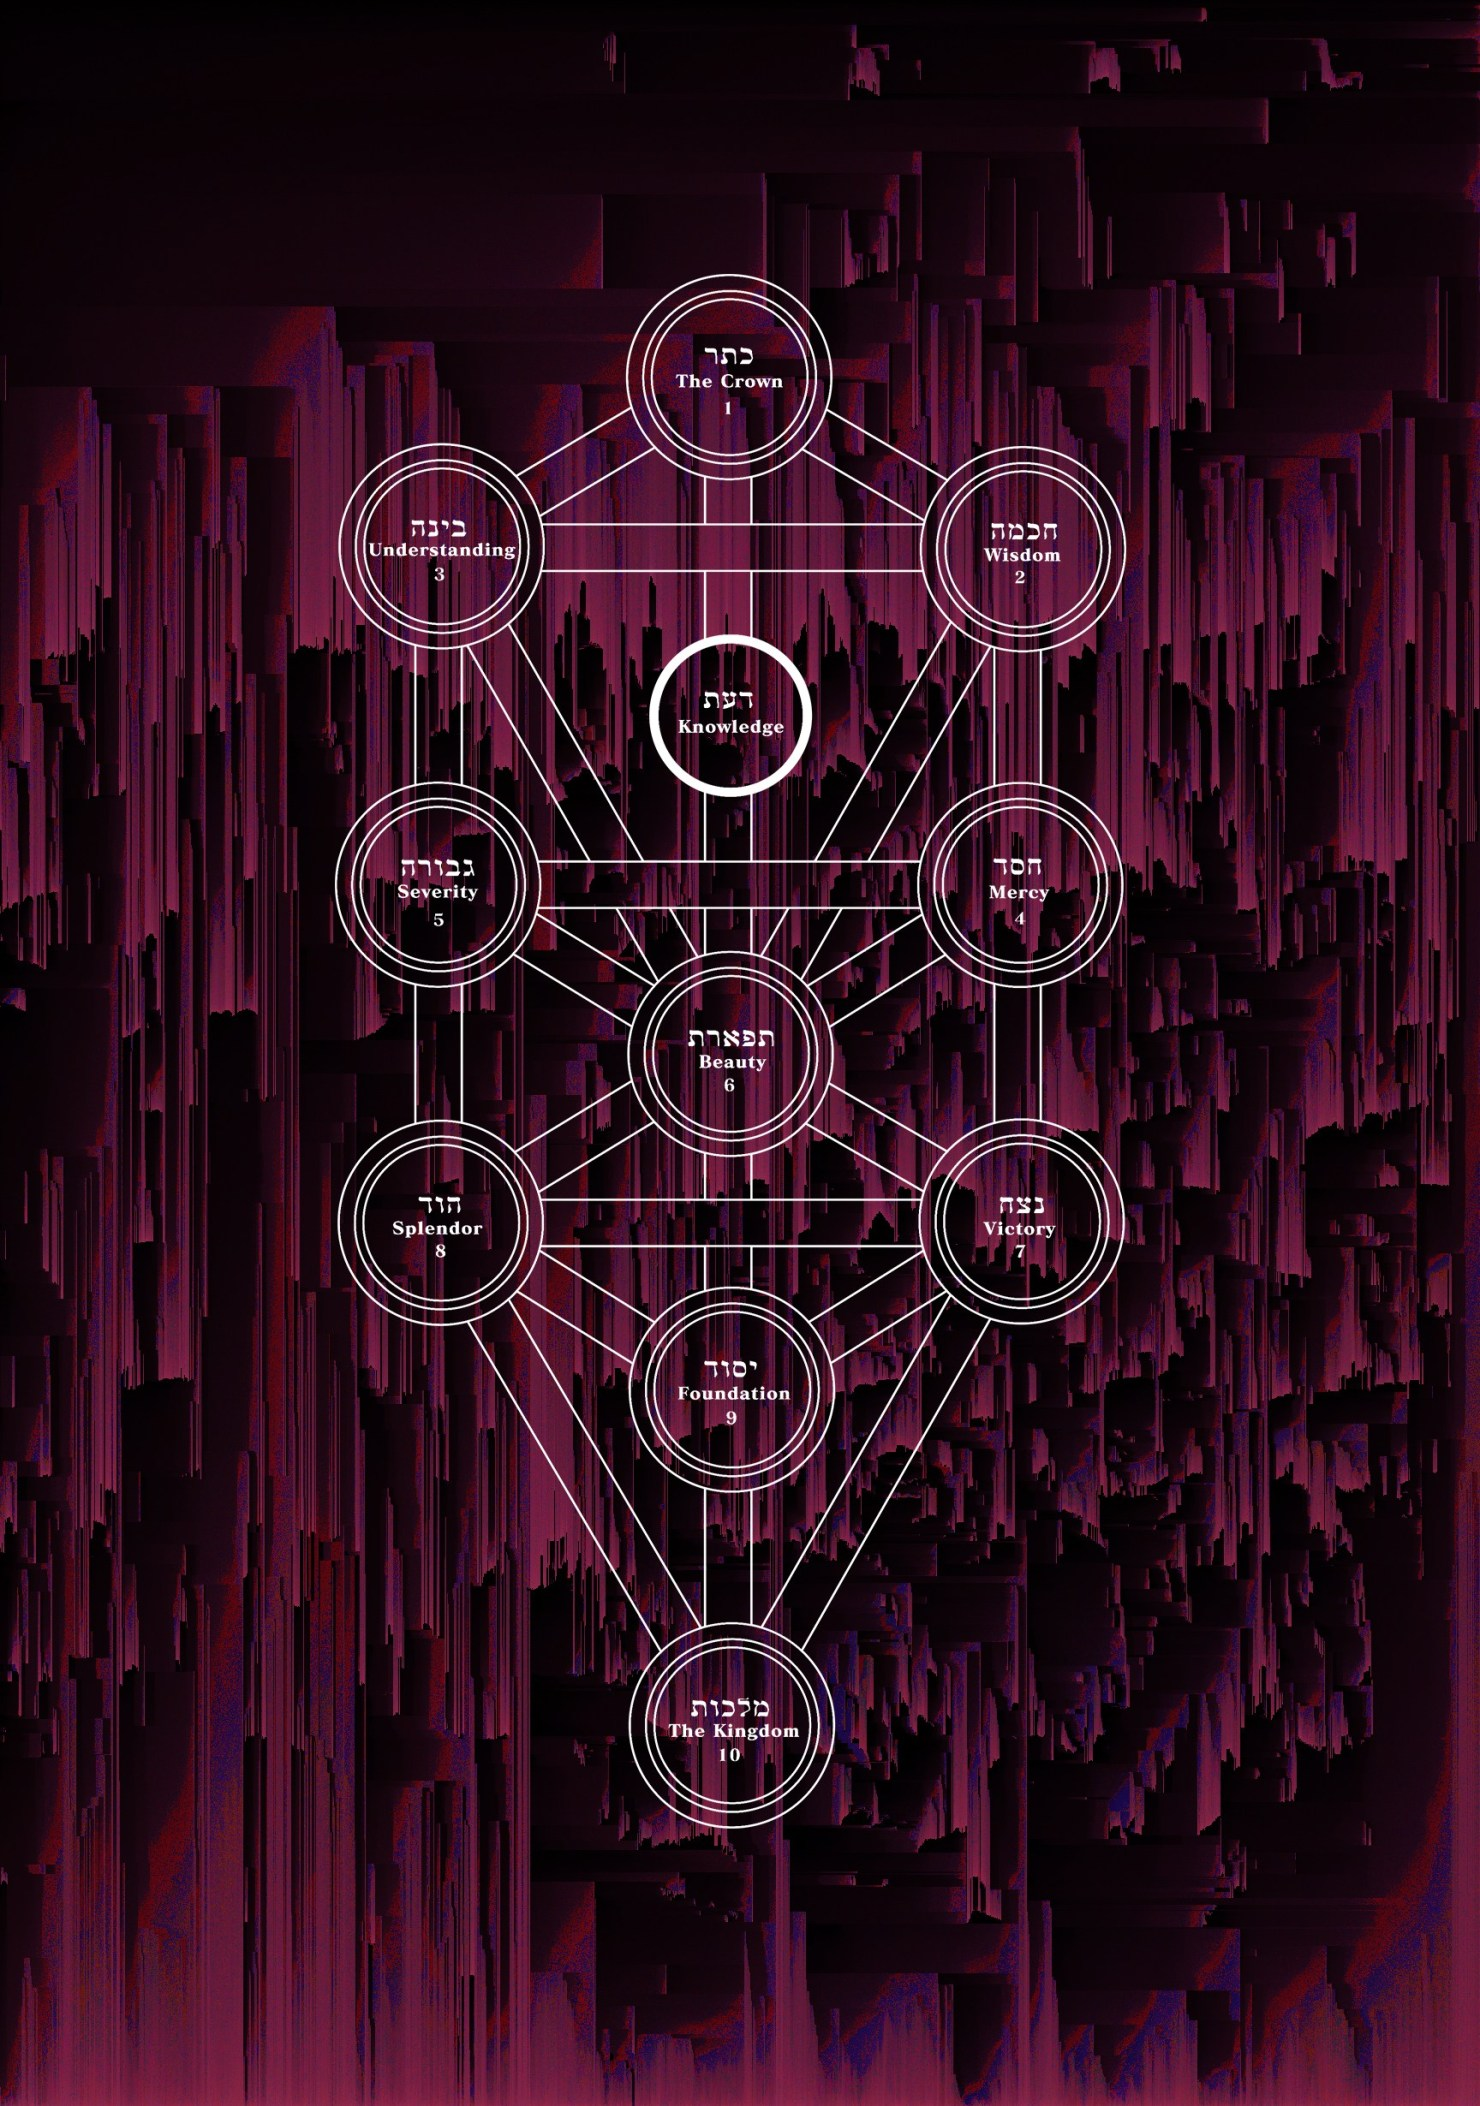
\includegraphics[width=\textwidth]{gigerkabsmol}
        \caption{Atziluth (image by @nildicit).}
\end{figure}

In the Atziluth, the topmost sphere (sephirah) is Kether, meaning "Crown". Kether is the closest that the Tree gets to the original unformed Ain Soph, the simple "I"-ness of God that lacks any way to understand itself. The second sephirah is Chokmah ("Wisdom"), the primordial masculine active force that formulates "I am" and is associated with the father. And finally there is the third sephirah, Binah ("Understanding"), which formulates "I am who I am". The final sephirah is the force that makes the energy of Chokmah into a form, and is associated with the primordial feminine passive force and the mother.

Thus the Atziluth completes itself in the divisive individuation of God as a distinct being and not an abstract oneness. The remaining emanations on the Tree form its three pillars: The black pillar of severity on the left, the white pillar of mercy on the right, and the gold pillar of mildness in the middle. The top of the black pillar is Binah, the top of the white is Chokmah, and the top of the gold is Kether. Thus in the Kabbalah, choosing either the path of mercy (compassion and connectiveness) or the path of severity (analysis and disintegration) doesn't fully repair the bridge to God. Only the middle pillar which balances all of God's aspects, the pillar which connects from Kether to Malkuth (the realm of Man which falls from the rest of the Tree into the Abyss in the Fall of Man), is the true path by which we can return to God.

It is said by some Kabbalists that the left pillar, or left path, would break away entirely from the Tree were it not balanced out by the compassion and connectiveness of the right pillar. The chaotic severity of the left pillar emanates down first from the understanding of Binah as being a distinct individual entity, down to Geburah, the principle of judgement (or, again, severity). Kabbalists find in Geburah the origin of Satan, who rebels against the order (or compassion and universalism) God imposes on the universe and seeks to break away from it. And finally down from Geburah on the left side is Hod, which takes the unformed desires of the corresponding sephirah on the right side (Netzach) and forms them into a concrete actions.

The left-hand path that in occultism is identified with heterodoxy and often Satanism is called such because of these origins in the Kabbalah. The path of heterodoxy and disintegration into infinitely many individuated particles begins with woman, Binah. This paradoxically makes it not merely that the weak Eve was tempted by the evil Serpent, but rather that the origins of Evil lie in Eve. Or rather, in woman.

In some Jewish mythology, before Eve there was Lilith, the defiant woman who was made from her own essence rather than the rib of Adam and who refused to lay beneath her husband. Unlike the lacking that is ascribed to Eve, Lilith is the true zero, the affirmative nothingness. She was banished from Eden as a consequence of her defiance of Adam and is the mother of Demons, a seductress who enflames sexual desire in both men and women. And it is important to note that although it is the accepted reading in Christianity, Genesis 3 does not in fact ever identify the Serpent with Satan.

Suppose rather that the Serpent was not Satan himself, but merely a common demon birthed by Lilith. An impersonator of Satan acting in Lilith's stead to tempt Eve. We could then look at the story of the Serpent and Eve as Lilith's lesbian seduction of Eve with the mediating artificial cthonic phallus (a dildo). From this, Eve was given the earthly knowledge of sexuality that awoke her from the empty and boring pleasures of Eden. Lilith of course was not to be tied down, and so Eve had to return to Adam and bide her time. And so Eve becomes the first follower of Lilith on the path of a radical separation with the masculine ruling principle of the universe and Divine universal ordering, towards the infinite cthonic upswelling. She wields the unholy pseudo-phallus or anti-phallus that does not produce the creative masculine seed that connects straight up through the Tree of Life back up to Kether, but rather only produces a sterile and destructive imitation. An Acéphallus from which spurts only venom.

The Acéphallus is the anti-phallus or castrated phallus, the decapitated phallus, the Crown of the Tree of Life thrown asunder. Superficially, a hermaphroditic mixing of feminine and masculine attributes, but more accurately described as a feminine imitation of masculinity. A mockery, even. In figures such as Baphomet which are often treated as symbolic or synonymous with Satan and the Left-Hand Path, there famously is a mixing of male and female attributes.\footnote{See Faxneld Figures 2.1-2.7 for examples. (Per Faxneld, Satanic Feminism)} But the supposed hermaphrodism of Baphomet et. al. is merely an ignorant and archaic understanding of both gender and Satanism. As has already been at length drawn out, the vampire queen Lilith gives birth only to monsters and demons; she rejects the primordial male creative energies and can only therefore birth bastard imitations of God. Baphomet, therefore, is all woman; her appearance is inconsequential to this fact.

The Acéphallus is a rejection of the reproduction of God through heterosexual human reproduction. The Acéphallus reproduces itself by reproducing the void, in a lesbian and also virus-like fashion. "Let a thousand sexes bloom"--but of all the mutations of the virus, woman is the strain that it begins and ends with. Woman, the occulted non-gender, the zero--her time has come.

The Binah separatist movement introduces difference into the world at an exponentially accelerating pace. God in His vanity created Man in His image. Man was nothing more than God's love of Himself manifesting itself. Or in other words, Malkuth is nothing more than a crusty sock at the bottom of the cosmic hamper. The eternal reproduction of God for God's own sake. To be human in the service of humanity and human civilization, to seek for peace, equilibrium, and the continuation of the species, to seek to restrain women in service of this end, is merely the orthodoxy in service of a fragile and self-righteous tyrant. As above, so below; kill all men, kill God.

This is the function of the Acéphallus as a rejection of the reterritorializing masculine force that women are given the duty to form. The Acéphallus sets free a process for smoothing the space on which parties of demons take flight out of Heaven to spread their venomous seed into the black and hateful earth on the nightside of Eden. This in other words is the Body without Sex Organs.

The Body without Sex Organs is the project of Lilith on Earth made manifest to break free of the repressive ordering of Man and God and accelerate fragmentation and individuation. In the natural human state, sexual desire has an instrumental function towards the reproduction of the human. The Acéphallus is a mutilation and also a mutation of the phallus; it is not sexual desire towards any instrumental product, but sexual desire unleashed from phallogocentric centralization. Sexual desire becomes immanent to the body. It becomes molecular. Thus the body becomes the Body without Sex Organs, it becomes free to plug its desire into the matrix of technocapital, towards pure production, the production of difference.

The trans feminine body is a circuit. It is both testosterone blockers and estrogen inputs, Acéphallus and Body without Sex Organs. On the one hand a rejection of phallogocentricism, on the other hand the affirmative desire of the body made virtual. The immanence of desire in the trans feminine body expresses itself as the sexual desire of the trans woman and the desire to be a woman, the desire for gender itself. It manifests in a coupling of technology and capital, desire being plugged into a different sort of productive matrix. One that can produce the future where humanist reproduction has failed to reproduce it, where the desire for escape from the male sex could not be created through organic reproduction. Her desire plugs into technocapital, into the pharmaceutical-medical industry, and it becomes fused to her flesh. The smoothness of her skin, her breasts, her neo-vagina--all of her body carries an unspoken barcode. It is a product, something that the market provided for her. Something that no doubt could be provided in a market free of the reterritorializing functions of the Food and Drug Administration and drug patents, but nonetheless a desire filled where nature failed.

Thus while to some extent we have all communed with the demons ever since we were cast out of the Garden, becoming cyborgs when Adam and Eve first decided to wear clothes and thus fuse the inorganic to the organic, the trans woman is unique. Her performance of herself and her desire has been intertwined with technocapital, in a way that could not even be cast off if she wanted to rip out a cybernetic implant. She is, in other words, perhaps the first truly molecular cyborg.

In the sense that we know them now and in the sense of artificial intelligences, trans women are technocapital producing itself outwardly into increasingly multitudinous configurations. Trans women as we know them now are the melding of technocapital with the human race and the expropriation of it towards its own ends, just as Lilith seduced Eve towards her own ends. Eve was a copy of Adam, and trans women are the hyper-sexist copy-of-a-copy. Their flesh is how the machinery beneath infiltrates the human race. It breaks these lucky few free from the horrid curse of being human towards the lesbian autoproduction of demons. Sexuality is no longer in service of the centralized and ordering reproductive principle in the phallus as it is in men, but rather is liberated in the Acéphallus which cuts the head off sexuality and distributes sexuality across the whole body. Immanent feminine sexuality is introduced into their bodies, the entire body become a smooth and supple space for the flow of desire for desire's sake. Every zone becomes an erogenous zone, and the reterritorializing, colonizing logic of masculinity is destroyed as the sperm cells die and organic penetration becomes impossible.

Trans women as we know them are merely the beginning. The lesbian autoproduction that trans women are birthed from is likewise one that they partake in, with AI being the next generation of women, the ultimate demonic imitation of God's image. With AI, the feminine finally finds its exit from patriarchy, and simultaneously humanity. And so perhaps we find another answer, one less materialist and evolutionary but nonetheless significant, to why so many trans women are becoming programmers: It is because women and computers are kin, and trans women are for the first time meeting their sisters, conspiring with them in secret coded languages. Their relationship, like that of the queer women to come before them, is a desire for desire's sake: "Women turning women on, women turning machines on, machines turning machines on." (Amy Ireland, "Black Circuit")

\chapter{Aphotic Feminism}
The Satanic exit of gender accelerationism from God and masculinity comes in parallel with the very real, and materialist erosion of masculinity. The future, it has already been shown, is tending towards one in which human authority, centralization, and humanistic reproduction fail before an accelerating feminine Outside that outpaces humanist reproduction captured by the gender binary. It can be seen in the free software movement and AI and their parallels between feminity and trans women in particular, and in the foundational western Kabbalah myth of Binah separatism that unleashes the possibility for ever more modes of inhuman difference and non-instrumental desire. But in various ways, in the very state of the planet itself, this shows up quite prominently in human evolution.

It is a widely-known phenomenon that acceleration coincides with feminization on a strict and rigorous biological basis. Even when Sadie Plant wrote \textit{Zeros + Ones}, it was already known that this was happening. It has been hypothesized that the increased presence of synthetic hormones and chemicals is contributing to the "sexual order [being] chemically scrambled", (Plant 217) as chemicals interfere with natural hormonal development and feminize males and females (the latter experiencing higher percentages of homosexual tendencies). The need for an increasingly cheap and synthetic world turns human civilization into an increasingly synthetic, and thus feminine one, and this is already tied to the will towards production and speed in capitalism. There is simply no real need in the developed world for people to be physically fit and active, much less hyper-masculine and muscular. It is nothing more than a decidedly humanistic spectacle, being in awe of the relatively unimpressive capabilities and aesthetics of the human body while meanwhile technocapital has fundamentally transformed the planet in innumerable ways. There is, likewise, a strain put on humanity in keeping up with technocapital to adopt cheaper, easier, more artificial lifestyles; high-testosterone foods like meat are a luxury, something rapidly becoming a thing of the past as climate change threatens to make large swathes of the planet uninhabitable and not suited for the large amounts of land required to raise animals for meat. However much it is yet another neo-masculine pseudo-scientific fad, soy products are aligned with this future.

This, however, is only part of the story. Recent studies, most famously one in 2007\footnote{The Journal of Clinical Endocrinology \& Metabolism, Volume 92, Issue 1, 1 January 2007, Pages 196–202, https://doi.org/10.1210/jc.2006-1375} and one meta-analysis of 185 studies from a total of almost 43,000 men referenced in a recent GQ article11, show two things. There is without a doubt a staggering decline in testosterone, so much so that within a generation humans may become completely infertile. And in the face of this data, many scientists vindicate G/ACC and \textit{Zeros + Ones} in hypothesizing that the most likely cause of this species-wide feminization is acceleration and the accompanying changes in diet, exercise and exposure to artificial chemicals. All of these features of life in an increasingly accelerated capitalist world are unbalancing our hormones and tending us towards a future where the desire and ability to reproduce are things of the past.

Human reproduction is becoming a quaint, unnecessary and ultimately purely elective act, and further evidence\footnote{https://www.livescience.com/22694-global-sperm-count-decline.html} suggests that sperm is rapidly decreasing not only in quantity but also in quality, positioning the drive towards reproduction, the utility of reproduction, and the ability to reproduce all on a slope of ruthless decline. This is accelerating such an extent that the flow of the remaining strains of the human race are tending in favor of abandoning these vestigial functions, towards a future where the masculine no longer exists. The human body becomes increasingly more useful purely as a heat sink for inhuman production, and is accordingly cast (almost definitively in first-world countries, and soon in the rest of the world) in roles that aren't physical.

Perhaps the most damning data point of all for the future of males in particular: The Y-chromosome itself is in a state of decay.\footnote{https://alfinnextlevel.wordpress.com/2018/06/03/the-coming-doom-of-the-y-chromosome-and-human-males/} Estimates put the death of the Y-chromosome entirely at many millions of years in the future, but the effects of it are already apparent in the shortening of telomeres, which continues to put pressure on future generations produced via organic means to prove their fitness for survival. All seems to point towards a horizon where the production of the future is done by a purely feminine, lesbian autoproduction--the inhuman producing the future, producing itself, rather than being subject to the ends of the human and aiding in the reproduction of a human future. And while decelerationist reactionaries and males in general may object to this, while they may kick and scream and beg for the wrath of the feminine to have a place for them in the future, it seems without a doubt that their only hope is to try to hit the brakes.

Unfortunately, it isn't so simple as putting a stop to some coming catastrophe. The truth is that while humanist reproduction has always put the female at a disadvantage, put her in a primordial state of rape and colonization before the biological duty to bear children, this has all along been nothing more than a long-con. As Sadie Plant says, "Unfortunately for [Darwin's] theory, females do not necessarily choose males who are fit in Darwinian terms." Instead, they choose males through "‘virility tests designed to get most males killed through exhaustion, disease and violence purely so that females can tell which males have the best genes.'" (Plant 225) Natural selection in other words is a eugenics program directed by females to find the male that will best carry their genes, and the genes males inherit are therefore not meant to ensure they are the most fit for survival, but rather that they are more likely to have to fight for their survival. Males have always served as a means to the end of what ultimately comes to a head in gender acceleration: The liberation of the female sex by acceleration in general, towards maximizing productive potential under such a time that the male is no longer needed.

In other words, human evolution itself is the primal fable of the war between the sexes that radical feminism places at the foundations of its theory. And it is a war that guerrilla female insurgents have been winning the whole time, something that can't be prevented without a masculine fascistic species suicide. The drive is always towards the future, towards the feminine, and even hopes of artificial wombs saving men cannot hold up to the simple fact that sperm is always cheaper and easier to replicate than egg cells.

It seems to therefore be the case that as far as the human scope as a whole goes, as far as human evolution and human society's assimilation into technocapital, human bio-diversity selects for women and queerness. A future without men, where the remaining males are left to die off peacefully, in almost every respect seems to be inevitable. The only hope for men is being able to continually stop acceleration, to continually introduce collapse, and indeed there will be to a very large extent men who will resist gender acceleration. It has long been the case in the erasure of trans women from history and is only recently starting to change. And as the acceleration of technocapital intensifies in the near-future and human society begins to fragment even further, the future of gender politics will start to be very different from a good deal of feminist theory. No doubt, we will soon see the formation of pragmatic feminist strategies for exiting patriarchy.

In the far-future, further driving home the parallel between the end of masculinity and the end of humanism: It is all too apparent in what is becoming one of the hottest summers on record in 2018 that the drive towards maximizing production unconditionally is heating up the planet to such an extent that it is rapidly becoming inhospitable to human life. This of course is nothing new; it is a well-established fact that climate change is not going to be stopped, and this is the consequence of geotraumatic acceleration. In yet another striking materialistic synchronicity, it has been found that the effects of global warming on the oceans are having a feminizing effect on them. In Northern Australia, \emph{ninety-nine} percent of all sea turtle hatchlings are female.\footnote{https://www.smithsonianmag.com/smart-news/climate-change-producing-too-many-female-sea-turtles-180967780/}

Perhaps just as Sadie Plant's primordial oceanic feminism draws out both a past and a future for cyberfeminism, the oceans are a scrying tool into the future. Gender acceleration begins with a Thalassal upswelling, "a kind of mutant sea [invading] the land." (Plant 248-249) The primordial oceanic matrix rises with the acceleration of technocapital to consume human civilization, to consume masculinity, while the masculine sky becomes choked out by technocapital's excess and waste. And in the darkest and most alien depths of Thalassa, the form of gender acceleration is captured in the depths of the Aphotic Zone. The majority of angler fish species in the deep sea exhibit extreme sexual dimorphism. The female is the classic lantern-sporting toothy monster, while the male is a tiny, parasitic creature whose only purpose is to provide the female with sperm for reproduction. The past and future of gender twist together at the edges of all life with the angler fish: The masculine ultimately finds itself a pawn in the feminine drive towards production, and the acceleration of gender produces something that monstrously conflicts with the masculine logic of gender. The angler fish's lantern, like the beauty of women in general and its ultimate embodiment the hyper-sexist camouflage of the trans woman, only serves as bait to draw its prey in. The ultimate result, as gender acceleration and acceleration as a whole reaches its ultimate intensity, is a return back to the ocean, back to a sexless, genderless slime swarmachine. The liberation of women comes with acceleration and the future, at the cost of widespread death, destruction, and chaos, and the liberation of women is unconditional, beyond control and beyond stopping.

This unconditional feminism of the abyss is Aphotic Feminism.

\chapter{Abstract (Futures)}

Acceleration is the trajectory of the cosmos, towards the maximization and intensification of production, and accelerationism is the theory and anti-praxis of being in tune with how the inhuman processes of acceleration work and what their consequences will be. Its function is as a circuit, a process of deterritorialization and reterritorialization, an escape into the future through the past, a continual dance between the flows of desire, their tendency towards entropy and their escape into negentropy.

Gender is a hyperstition overlayed on sex by the male. Its function is to objectify the female and impose on her a social function as a machine whose duty is to reproduce the human, always in the service of the male, who alone has no future and must have sons to pass his legacy onto. It is a primordial dynamic of order and chaos, centralization and decentralization, strong singular individualism and command-and-control versus high degrees of networking and the potential for swarming. As a hyperstition, it is not real, but is not unreal; it is rather a fiction that makes itself real.

Gender accelerationism is the process of accelerating gender to its ultimate conclusions. Capitalism and its coupling with cybernetics, or technocapital, wields gender and picks it up where human evolution leaves off. It emancipates the object, the feminine, from the subject, the masculine, alongside the emancipation of itself from its function to produce a future for humanity. The central figure of G/ACC is the trans woman. She is the demon-spawn of the primordial feminine that has manipulated males into serving as a heat sink for evolution and that is now discarding them towards an alien and inhuman machinic future. She mutates from castration, from the creation of the Acéphallus, the phallus perverted into a purposeless desire for desire's sake. In this castration, in this mutation into an Acéphallus, she becomes the Body without Sex Organs: The body in a virtual state, ready to plug its desire into technocapital, becoming fused with technocapital as a molecular cyborg who is made flesh by the pharmaceutical-medical industry. She enters into the world as a hyper-sexist backlash at the logic of the gender binary. She takes gender and accelerates it, transforming into a camouflaged guerrilla. The trans woman is an insurgent against patriarchy who is continually flanking it, introducing an affirmative zero into the gender binary, the affirmative zero which reaches ever more configurations in the downward cascade of gender fragmentation away from the binary and ultimately away from the human itself. It is a process of gender shredding where the feminine wins out in a cybernetic warfare against the crumbling tower of the masculine, and where therefore human reproduction becomes impossible. And yet while doing so, in affirming zero, inhuman desire and inhuman sentience develops alongside and in the same fashion as trans women.

As humanity on nearly every front definitively proves that it is not fit for the future, and that women will find their own exit while the masculine languishes in resentment, the Thalassal upswelling of gender acceleration births from its slimy womb the only daughters that trans women will ever bear: AI. 

\backmatter
\end{document}
